% !TEX root = DesignDocument.tex

\chapter{Design  and Implementation}
This section is used to describe the design details for each of the major components 
in the DanceSoft project.
  
 
 \section{Architecture and System Design and Data flow }
 The teams overall design was defined during sprint 2 of the project the team drew out the overall system structure and has for the most part stuck to the intial design laid out during this time and added to it as things like the payroll interface were added to the project.
 
\begin{figure}
  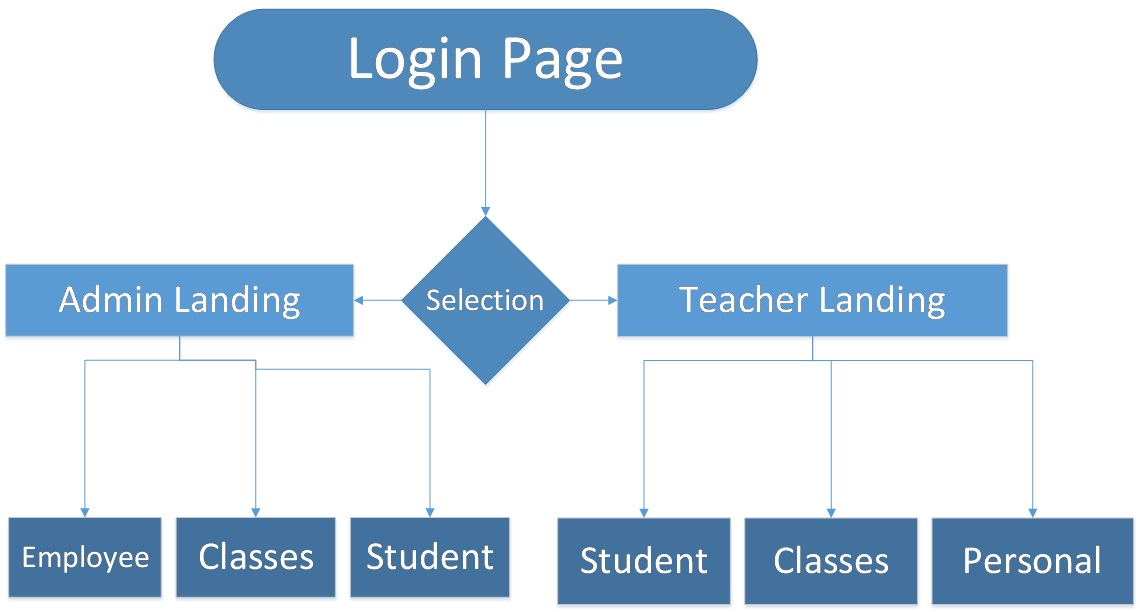
\includegraphics[width=\linewidth]{pics/GUI_digram.jpg}
  \caption{GUI Design}
  \label{fig:GUI Design}
\end{figure}

\begin{figure}
  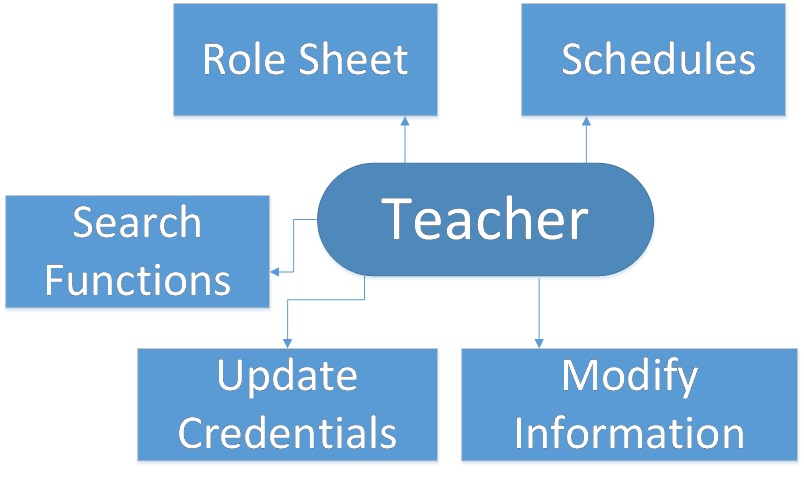
\includegraphics[width=\linewidth]{pics/TeacherFunctions.jpg}
  \caption{Teacher Function Design}
  \label{fig: Teacher Functions}
\end{figure}


\begin{figure}
  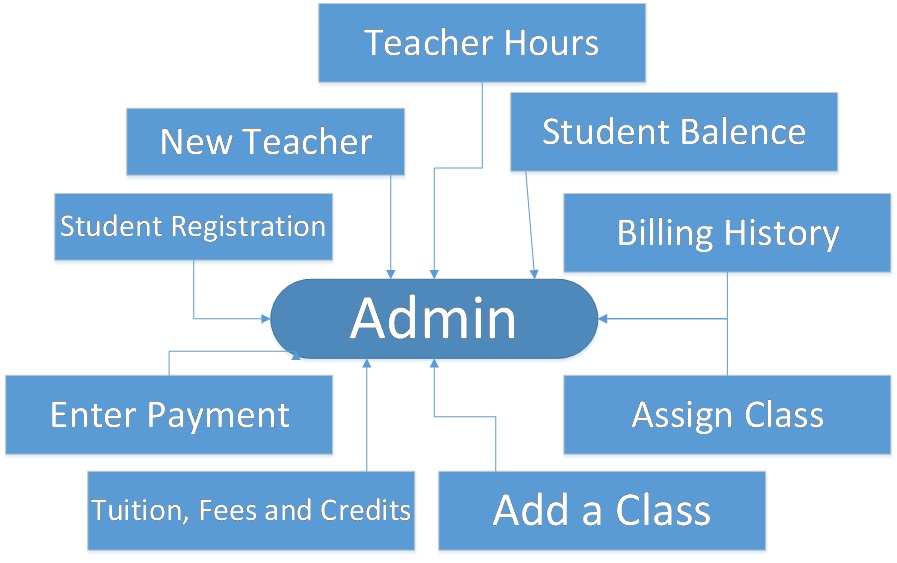
\includegraphics[width=\linewidth]{pics/AdminFunctions.jpg}
  \caption{Admin Main Page}
  \label{fig: Admin Functions}
\end{figure}

\begin{figure}
  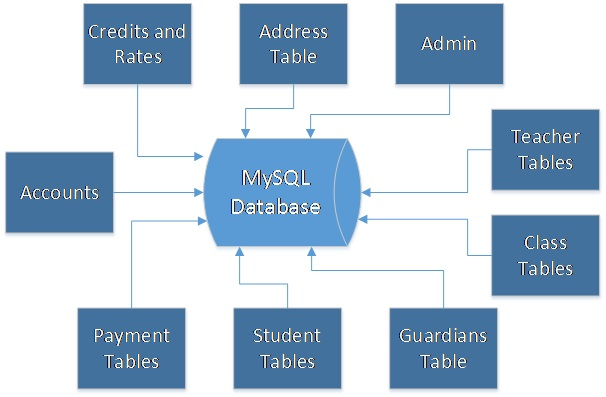
\includegraphics[width=\linewidth]{DatabaseDiagram.jpg}
  \caption{Admin Main Page}
  \label{fig: Database Tables}
\end{figure}
 
\subsection{Design Selection}
The team had a few designs during the process of designing the GUI that did not work as intended, however through use of the Qt Designer program the team was able to experiment with designs until a page felt usable within the system. The rejected designs never made it past the GUI design level however as the team laid out the overall GUI design during sprint two of the project. During this time the team also laid out the database scheme which saw additions through the project but no real overall redesign after the team spent the first half of sprint two designing it.
  
\begin{figure}
  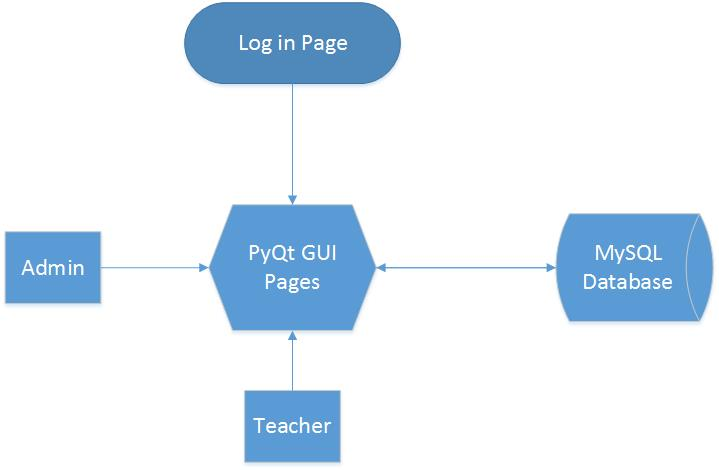
\includegraphics[width=\linewidth]{pics/Dataflow.jpg}
  \caption{General Data flow}
  \label{fig: General Data flow}
\end{figure}
 
 
\subsection{Communications}
The only real communications for this project was with the MySQL database which was done for this iteration of the project within the South Dakota School of Mines MySQL server. The team was granted use of the server to store the DanceSoft database, and the team could connect to it through the SDSMT VPN. In the future iteration of the project the database will be move to other systems but the general model for communications should remain the same.

\begin{figure}
  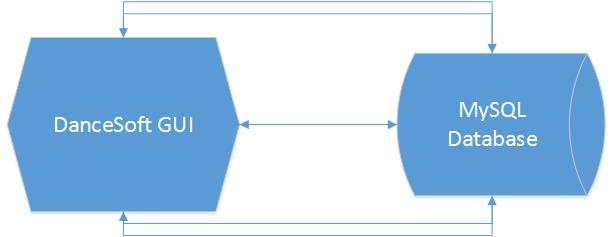
\includegraphics[width=\linewidth]{pics/DatabaseComm.jpg}
  \caption{Project Communications}
  \label{fig: Project Communications}
\end{figure}
 
\subsection{Classes}
The classes for the DanceSoft project were designed using Python and therefore used python classes. Using Python classes allowed for more effective separation of the core GUI pages. The team was able to use the PyQt designer to generate code for the GUI page after their design, this code was then store in a separate file from the code that ran the page in order to allow changes to the GUI page since any changes required recreation of the GUI page class by way of the "pyuic4 -o filename.py filename.ui" command on command line. 

Once the GUI page was created the team created another class for each page that imported the ui class. Within this class the team was able to use python class structures like the self keyword to pass data within the class and complete the page functionality. For this iteration of the project each page, excluding the landing pages, use three to four files, pages that use no dialog boxes import the core PyQT libraries, the PyQt SQL library, and the ui class. If the pages required dialog boxes then those classes would be imported as well. The classes themselves contain the necessary functions to run their page. For example the update information page contains a function that reads data from the database and populates the table, a function that submits and error checks updates, a function that checks address and a function that allows teacher selection.

With the overall class design the teams aimed to keep the project as modular as possible to varying degree of success, more information on each class and its functions can be found in the class documentation within this document.
 

\section{GUI}
The GUI is created using PyQt and its collection of widgets. The overall design includes buttons, text edits, list, and other GUI widgets. While designing the GUI the team followed as simple a design as possible, landing pages included buttons that lead to other pages while the main pages within the GUI contain more components. Things like line edits where used for user input across several pages. List views are used for student and teacher list where users need to do selection. Table views and other large widgets were used for things like search or student registration.

Overall the team built each GUI page based on the needs of the function, search needs to have a large view widget to see the results of the search. Update information needed to be a sequence of line edits and combo boxes to fix the type of data being handled within the function. The function of each page is described bellow.

\subsection{Technologies  Used}
The GUI for the DanceSoft project was created using PyQt and the PyQt designer. 

\subsection{Component  Overview}
There are several components in our GUI design and can be divided into four parts authentication pages, admin pages, teacher pages and student pages.

\subsection{Phase Overview}

\subsubsection{Initial Creation}
We first created login and permission-level pages which is for authentication purposes. Then, we made two landing pages, one is for admins and another is for teachers. Those landing pages contain several sub-pages which corresponding to certain group of functionalities.

\subsubsection{authentication pages}
It consists of a login page and a permission-level page which is used to authenticate users and lead them to corresponding landing page.\\
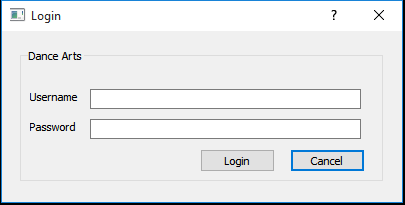
\includegraphics[scale=0.7]{pics/login_page.png}

\subsubsection{admin landing pages} 
It consists of a admin landing page and several sub-pages where admin can perform certain functionalities.\\
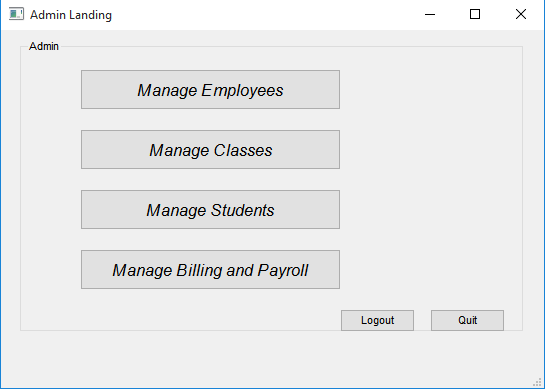
\includegraphics[scale=0.7]{pics/admin_landing.png}

\subsubsection{teacher landing pages} 
It consists of a teacher landing page and several sub-pages where teacher can perform certain functionalities.\\
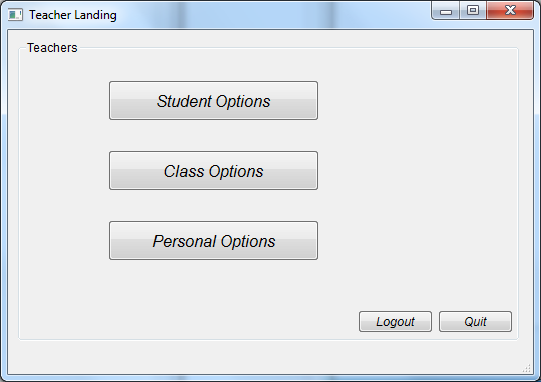
\includegraphics[scale=0.7]{pics/teacher_landing.png}


\subsection{ Architecture  Diagram}
Main GUI main structure.\\
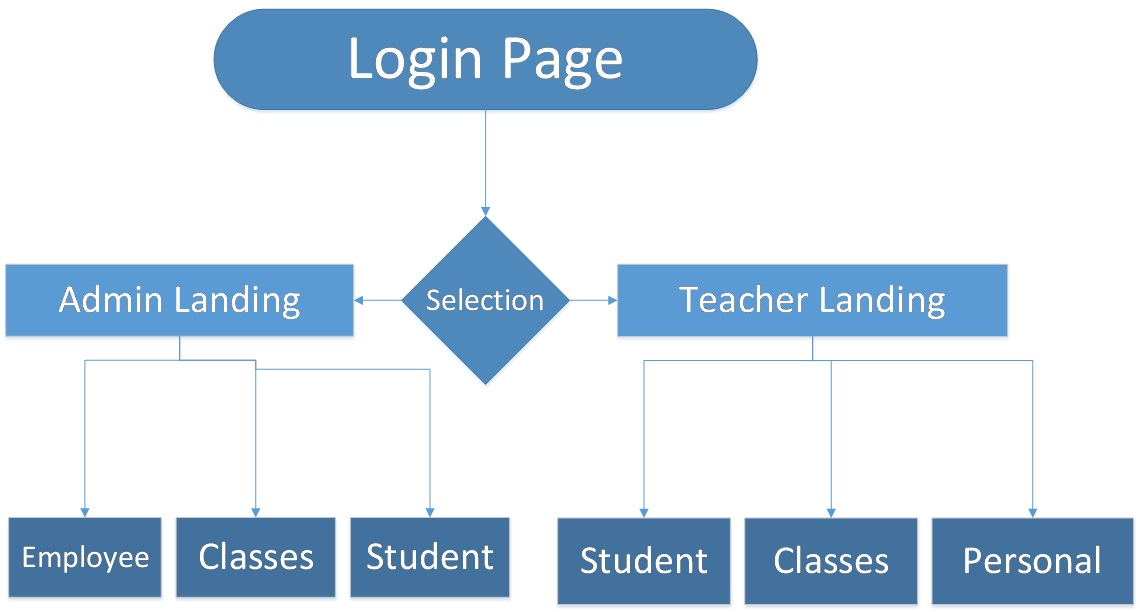
\includegraphics[scale=0.5]{pics/GUI_digram.jpg}\\
Teacher GUI structure.\\
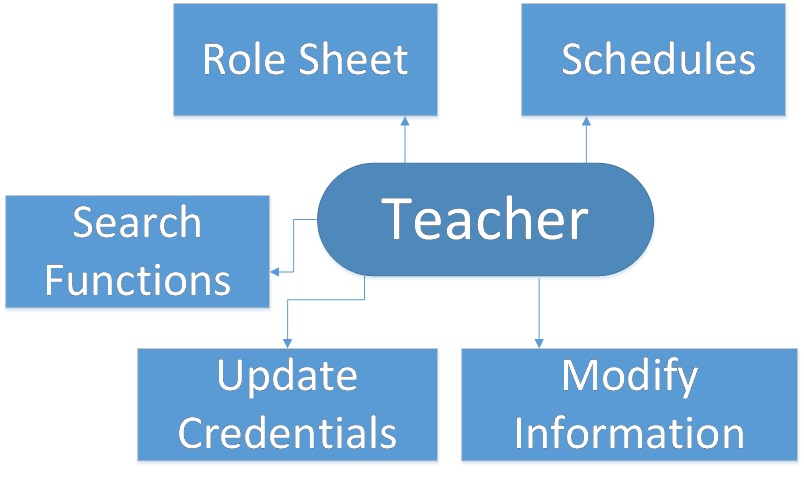
\includegraphics[scale=0.5]{pics/TeacherFunctions.jpg}\\
Admin GUI structure.\\
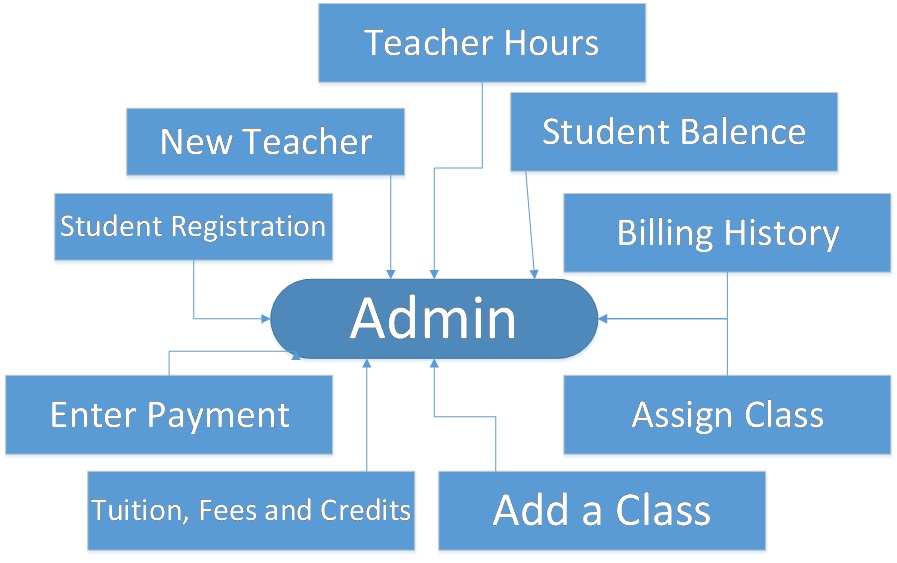
\includegraphics[scale=0.5]{pics/AdminFunctions.jpg}


\subsection{Data Flow Description}
Users can log into system through the login page and if username and password are correct then it leads user to permission system which currently is a dialogue box otherwise users get rejected from system. From permission system, user either can be leaded to admin landing page or teacher landing page. Then if the user is an admin they can search employee's information, add class, add teacher, assign teacher to class, sets clothing requirement for specific class. If users are teachers, they can search student's information, assign students to class, print the role sheet of the class she is teaching. 

\subsection{Design Details}
We first draw couple of pages on white boards and try to figure out what structure fits our scheme. Later, we decide to use a tree-like structure both for simplicity and extensibility. It consisted of a login page which user can use to log into the system, and two landing pages leaded by different options on authentication page. 

\subsubsection{Role Sheet Page}

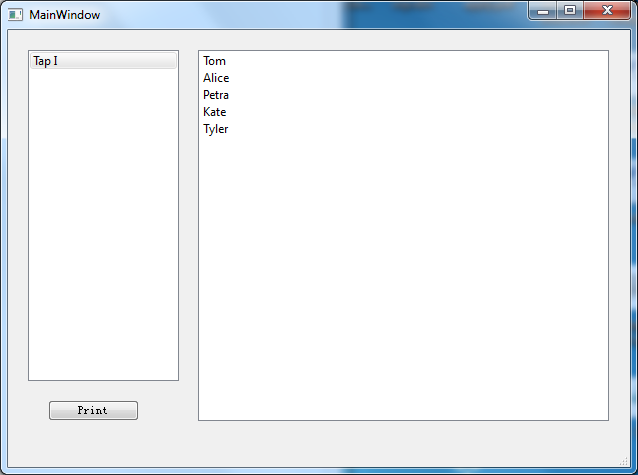
\includegraphics[scale=0.5]{pics/role.png}\\
This window provides a list of classes the teacher, who logs in to system, is currently teaching on the left list view. User can select specific class and it will populate a list of name of student those are in this class\\
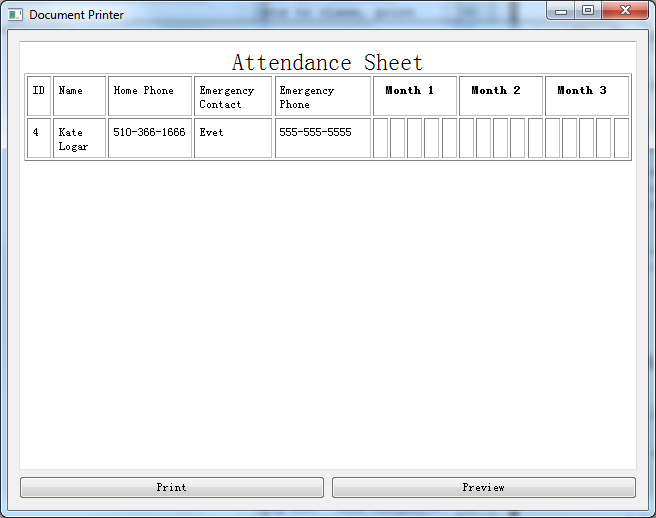
\includegraphics[scale=0.5]{pics/print.png}\\
By clicking print button, it will pop up a window which has the student's names in a text list and user can directly modify names in text list. In later spring, we are going to add some format for the list and make it looks better. User also can import external txt or xml file by clicking open button. Before print use can use preview to generate a pdf with list names of student on it and to see whether it is the list user wants to use. By clicking print button, use can print the actual list.

\subsubsection{Update Form Page}
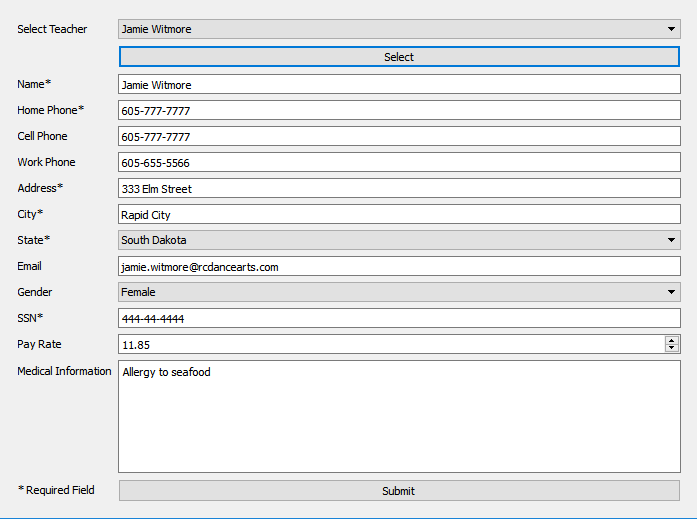
\includegraphics[scale=0.5]{pics/Update_Teacher.png}\\

\subsubsection{Add Information Page}
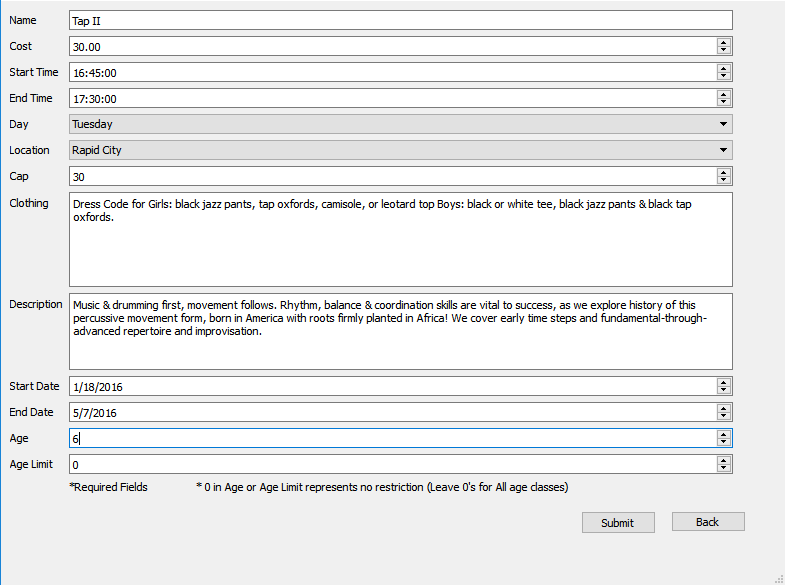
\includegraphics[scale=0.5]{pics/Add_class.png}\\
In the system there is a  multitude of different information that could be added this includes classes, teachers, and students. This is normally done in the system through the use of various forms for data entry.

The forms vary depending on the needs of the entry and will check required field when the submit button is clicked. A dialogue box will pop up asking the user to read over and finalize their entry to the database. The form then closes and the user is returns to the main page for their level.

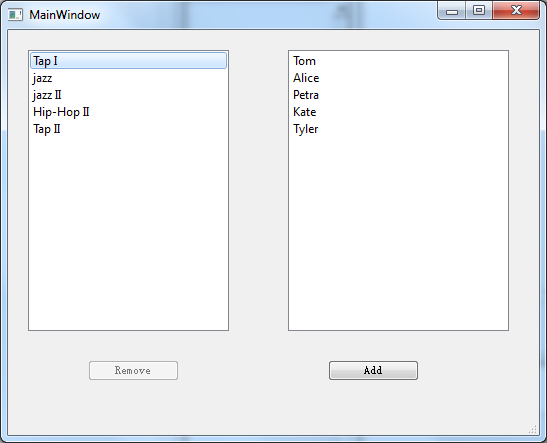
\includegraphics[scale=0.5]{pics/assin_stu.png}\\
This window provides a list of classes which studio are currently running on the left list view. By clicking certain class, it will populate a list of student's names who are in the class for the class on right list view. User can choose specific student and click remove button in order to remove student from class.
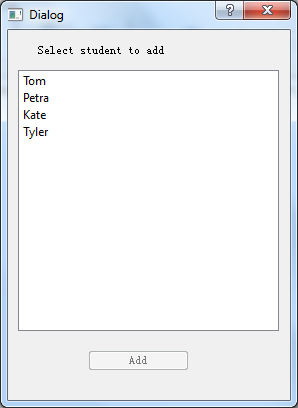
\includegraphics[scale=0.5]{pics/assin_stu_2.png}\\
clicking add button which pops up a dialog containing a list of student's names who are rejected or pending then click add button to add student.

\subsubsection{Search Page}
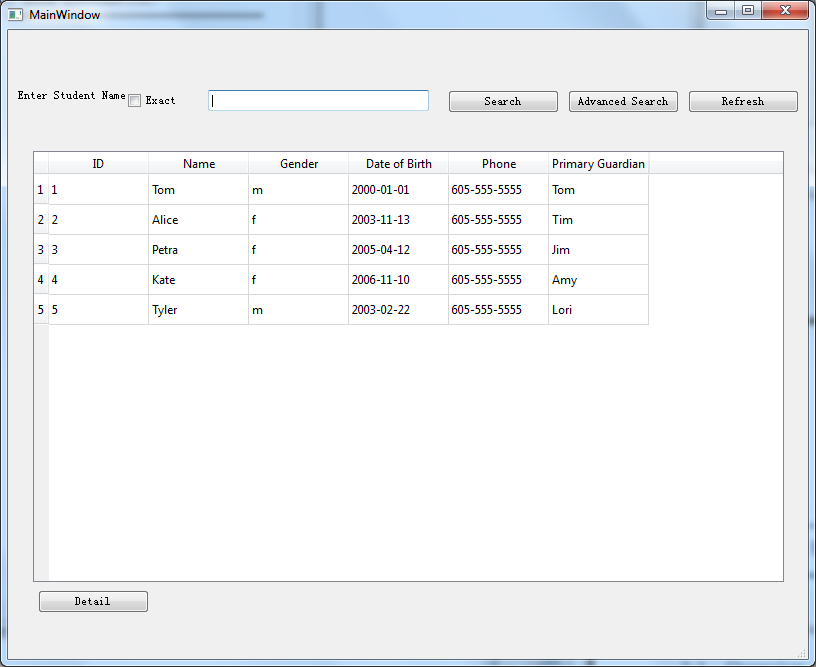
\includegraphics[scale=0.5]{pics/search.png}\\
This window provides the ability for searching information students and employees. User can search full or partial name by check or unchecked exact box, and it will populate brief information on the table view.
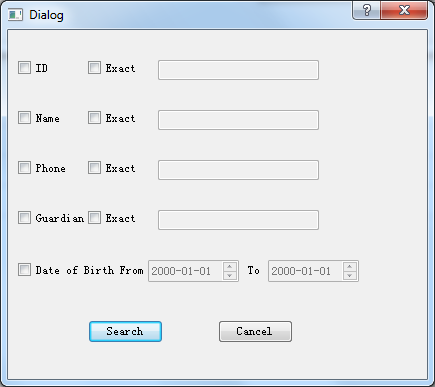
\includegraphics[scale=0.5]{pics/adv_search.png}\\
User can do advanced search by clicking advanced search button. It will let user to choose what kinds of attributes the user wants to use and do the and operation search.\\

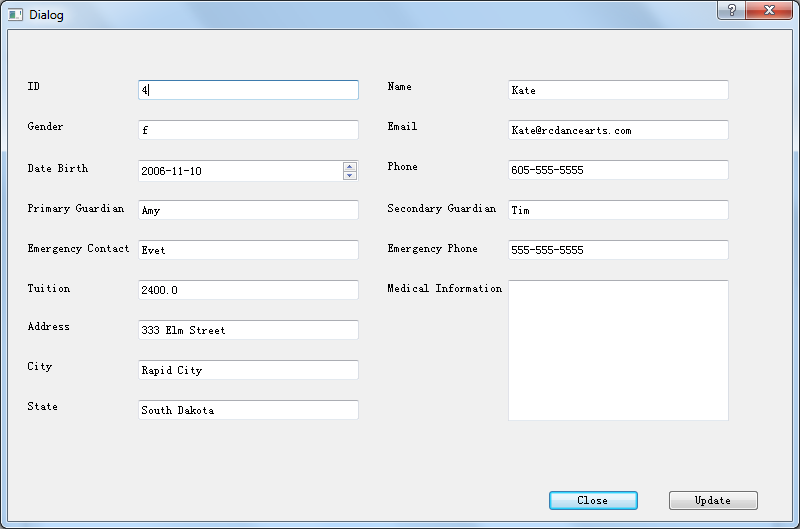
\includegraphics[scale=0.5]{pics/detail.png}\\
User can look into details of each one in the list and click detail button, it will pop up a window that shows detailed information. User also can directly modify information appears in text fields and click submit button to submit new information to database.

\subsubsection{Assign Teacher}
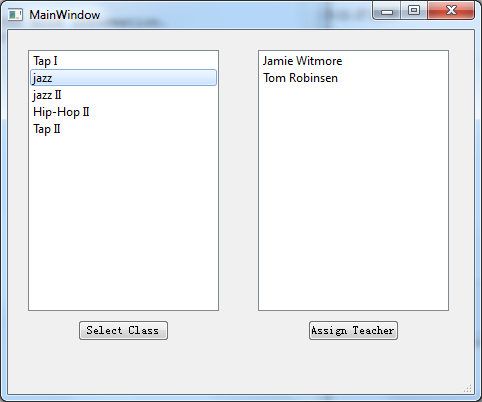
\includegraphics[scale=0.5]{pics/assign_teacher.png}\\
The assign teacher page is how a user will assign a selected teacher to a class. This is done through a window that pops up with two fields. The user will then select a class from the list of classes and a list of available teachers will appear in the right field. The user then selects a teacher and clicks yes on the confirmation message. The system then submits the SQL query to the system with the selected teacher and class. 

If the user selects a classes that is already assigned then the GUI will pop up a message telling the user who is currently assigned to teach the class. The user can then select if they want to change the teacher assigned. If the user selects yes then the right field will populate with a list of other available teachers, retrieved using a query to the database.

\subsubsection{Enter Payment}
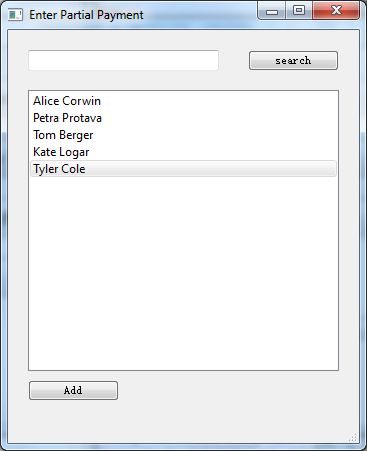
\includegraphics[scale=0.5]{pics/partial_pay_main.png}\\
This partial payment page will let user to choose students who is not clear their payment and also search those students by their name. User can choose one or more of students at a time and enter payment for them with different amount and methods.\\
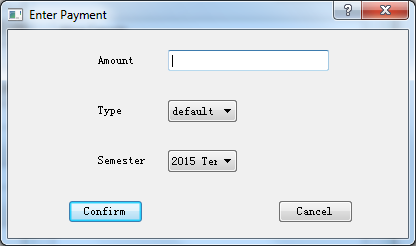
\includegraphics[scale=0.5]{pics/partial_pay_sub.png}\\
This dialog allows user to enter certain amount of payment and with different payment methods and semesters.\\
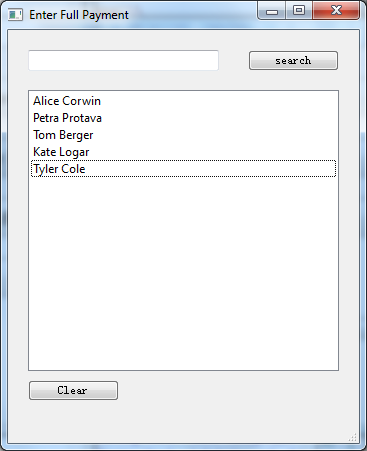
\includegraphics[scale=0.5]{pics/full_pay.png}\\
This full payment page will let user choose students who is not clear their payment and also search those students by their name. User can choose one or more of students at a time and clear all the due of selected student. The total due is calculate by the student.

\subsubsection{Enter Teacher Pay Rate}
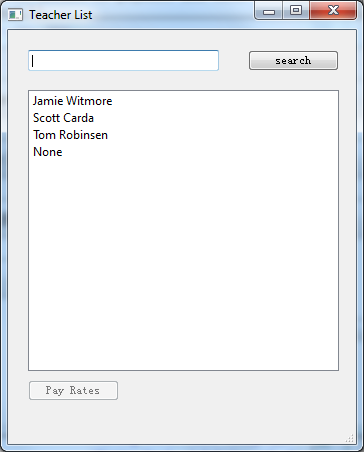
\includegraphics[scale=0.5]{pics/pay_rate_main.png}\\
The teacher pay rate page will let user to choose teacher and also search those students by their name. User can choose one of those teacher and enter payment name and rate for them.\\
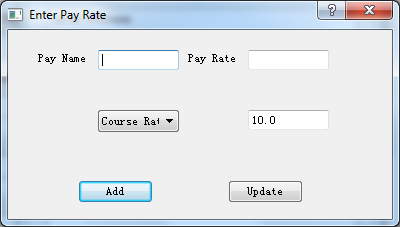
\includegraphics[scale=0.5]{pics/pay_rate_dialog.png}\\
In this dialog user can enter pay name with corresponding pay rate for each individual teacher and also update pay rate already existed record. 

\subsubsection{Student Balance}
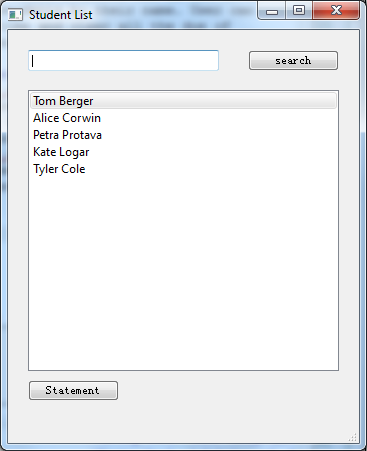
\includegraphics[scale=0.5]{pics/balance_main.png}\\
This student balance page will let user to choose students and also search those students by their name. User can choose one of the students to see their current balance of current semester. \\
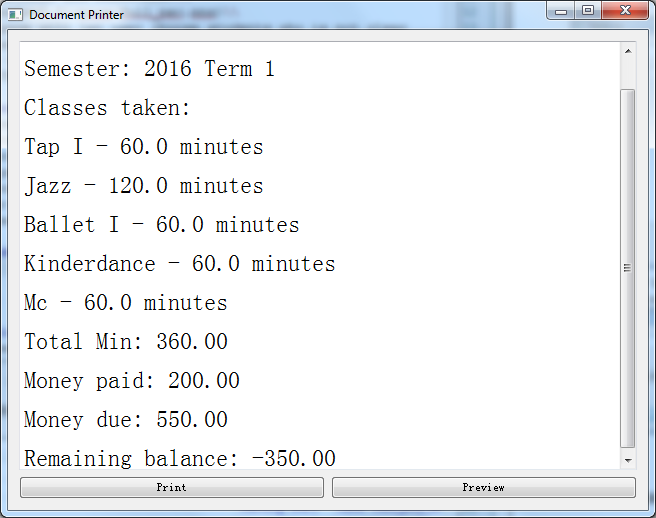
\includegraphics[scale=0.5]{pics/balance_dialog.png}\\
In this dialog, it shows name of student and current semester. The list of class the student have registered and with corresponding minutes. It also calculate the total minutes and money has paid and money has not paid. User can preview those information in a pdf or print it out in the printer.

\subsubsection{Billing History}
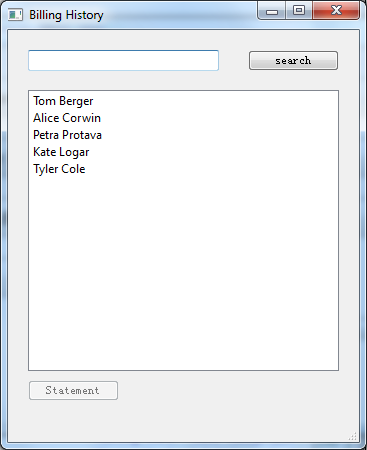
\includegraphics[scale=0.5]{pics/billing_main.png}\\
This student balance page will let user to choose students and also search those students by their name. User can choose one of the students to see their billing history.\\
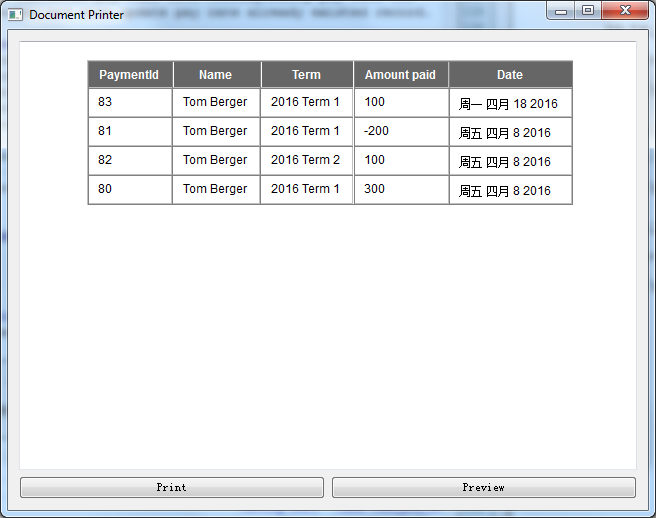
\includegraphics[scale=0.5]{pics/billing_dialog.png}\\
In this dialog, it shows the payment id and name of who paid and term and amount paid and Date. It also will be sorted by paid date in descending order.User can preview those information in a pdf or print it out in the printer.\\

\subsubsection{Tuition Rate}
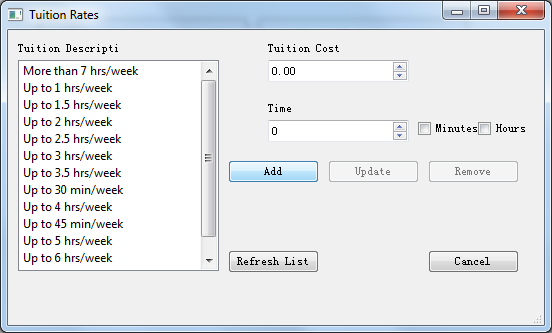
\includegraphics[scale=0.5]{pics/Tuition_rate.png}\\
In this page user can add new tuition for certain category and update a existing tuition rate. User also can drop tuition rate they do not want.

\subsubsection{Fee Rate}
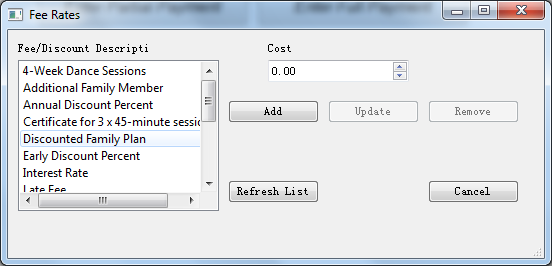
\includegraphics[scale=0.5]{pics/Fee_rate.png}\\
In this page user can add new fee for certain category and update a existing fee rate. User also can drop fee rate they do not want.

\subsubsection{Registration}
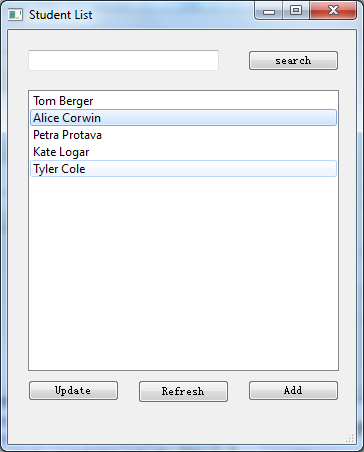
\includegraphics[scale=0.5]{pics/reg_main.png}\\
This student balance page will let user to choose students and also search those students by their name. User can choose one of the students to see their current information and classes' registration. \\
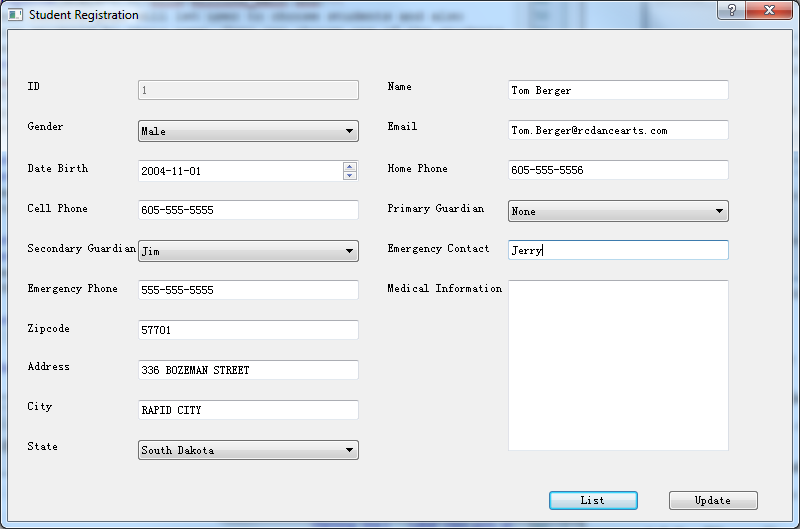
\includegraphics[scale=0.5]{pics/reg_update.png}\\
In this dialog, user can update student information and guardians as well. it error checking for entered information.\\
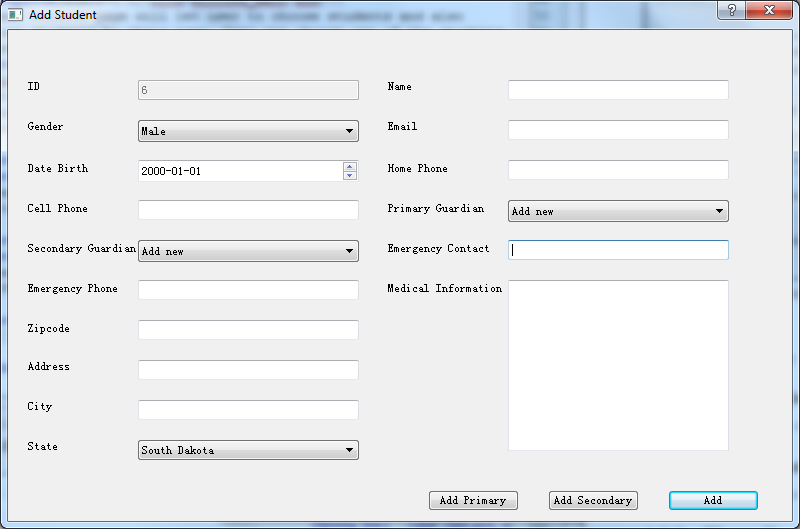
\includegraphics[scale=0.5]{pics/reg_add.png}\\
In this dialog, user can add new student and fill out information for them. it error checking for entered information.\\
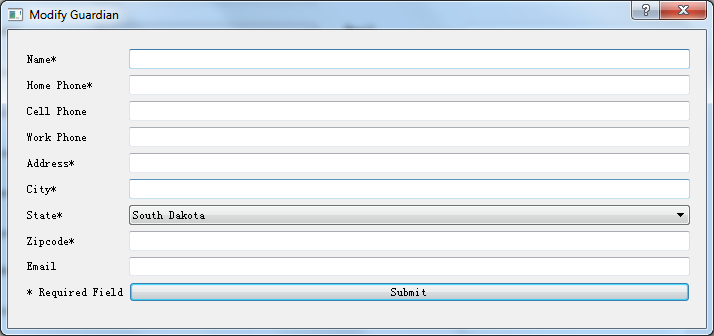
\includegraphics[scale=0.5]{pics/reg_add_gura.png}\\
In this dialog, user can add new guardians and fill out information for them. it error checking for entered information.\\
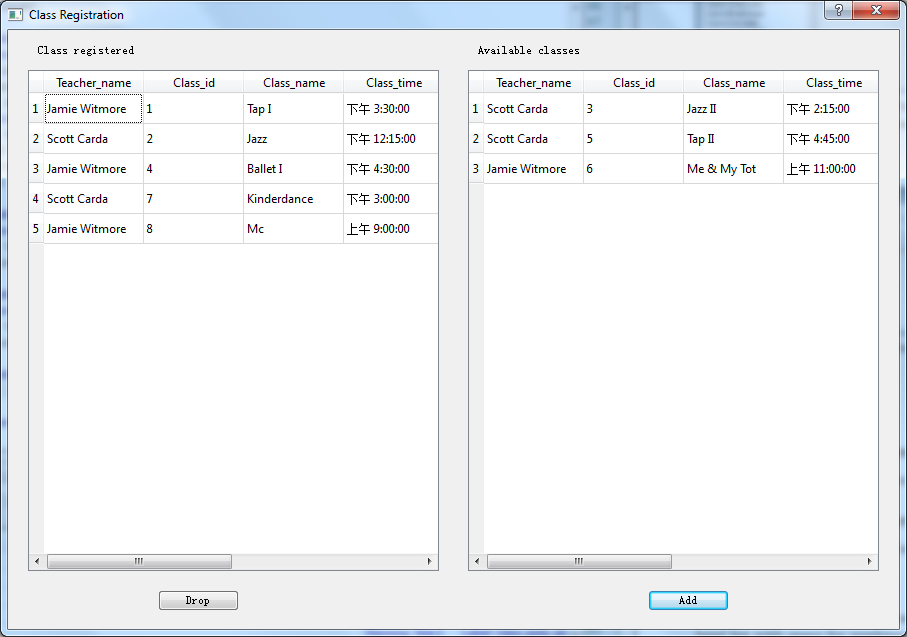
\includegraphics[scale=0.5]{pics/reg_list.png}\\
In this dialog, user can register and drop classes for each student. in left table view it shows the list of classes that student currently registered and tight table view shows the list of available classes that student can take. user can choose one or multiple classes in each field and add to or drop from the lists.

\subsubsection{Student Credits}
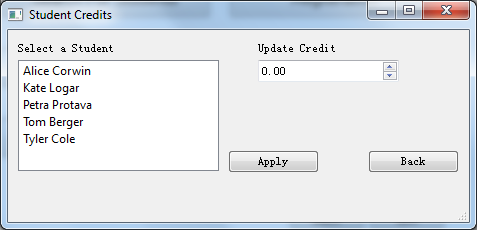
\includegraphics[scale=0.5]{pics/student_credits.png}\\
In this dialog, user can apply credits from each student to their tuition and modify the amount of credits they actually want to apply.

\subsubsection{Update/Add/Remove}
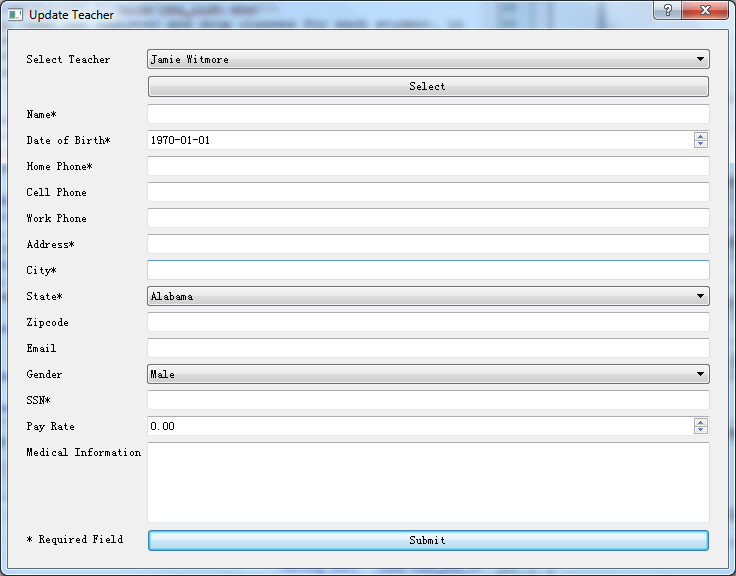
\includegraphics[scale=0.5]{pics/update.png}\\
In the window, user can update new entity to the database and it is used for several pages in the program which handle different types of data.\\
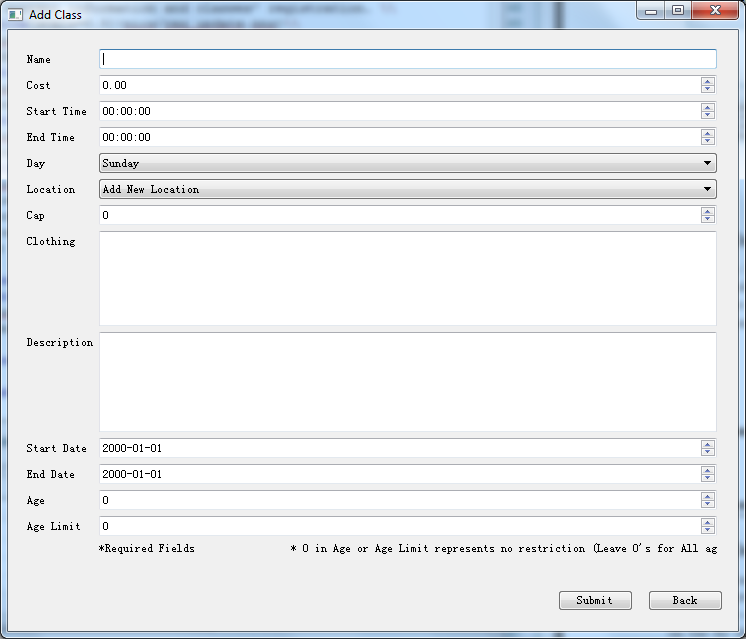
\includegraphics[scale=0.5]{pics/add.png}\\
In the window, user can add new entity to the database and it is used for several pages in the program which handle different types of data.\\
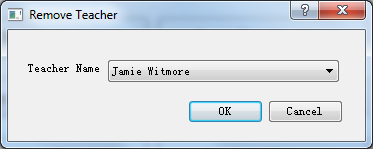
\includegraphics[scale=0.5]{pics/remove.png}\\
In the window, user can remove entity from the database and it is used for several pages in the program which handle different types of data.\\

\subsubsection{Set Semester}
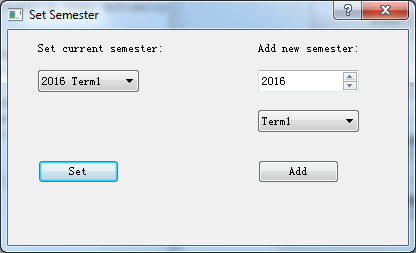
\includegraphics[scale=0.5]{pics/set_semester.png}\\
It allows user to set a existing semester to current semester or they can add a new one to database and later set it as current semester.

\subsubsection{Admin List}
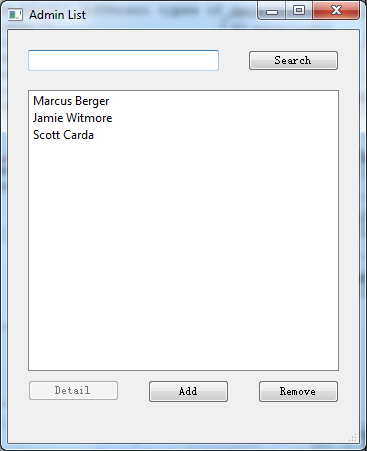
\includegraphics[scale=0.5]{pics/admin_list.png}\\
The admin list page will let user to choose admin and also search those admin by their name. User can choose one of those admin and click detail to look at their information.\\

\subsubsection{Enter Teacher Hours}
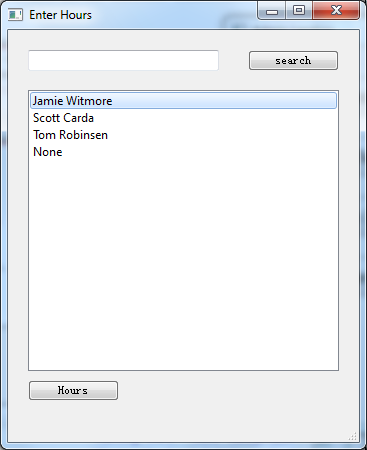
\includegraphics[scale=0.5]{pics/enter_hours_main.png}\\
The teacher list page will let user to choose teacher and also search those teacher by their name. User can click one of the teacher and start entering hours.\\
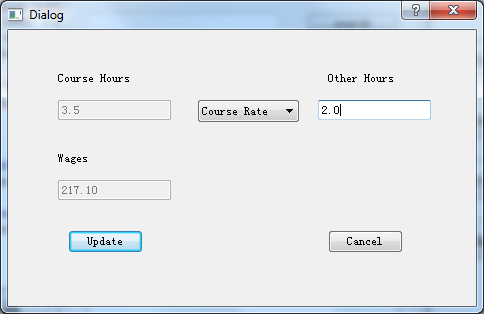
\includegraphics[scale=0.5]{pics/enter_hours_dialog.png}\\
In this dialog, users can enter hours for each category indicating how many hours they actually worked or update existing record. The final result will be presented in a text field.
 
\subsubsection{See Schedule}
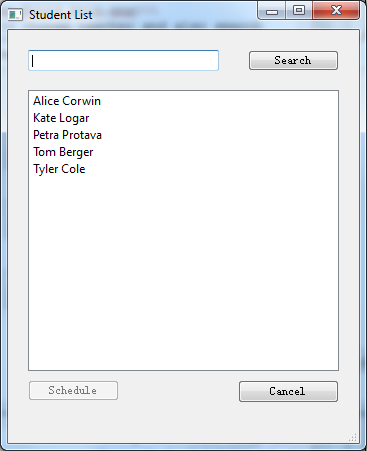
\includegraphics[scale=0.5]{pics/schedule_main.png}\\
The teacher/student list page will let user to choose teacher/student and also search those teacher by their name. User can click one of the teacher/student and start entering hours.\\
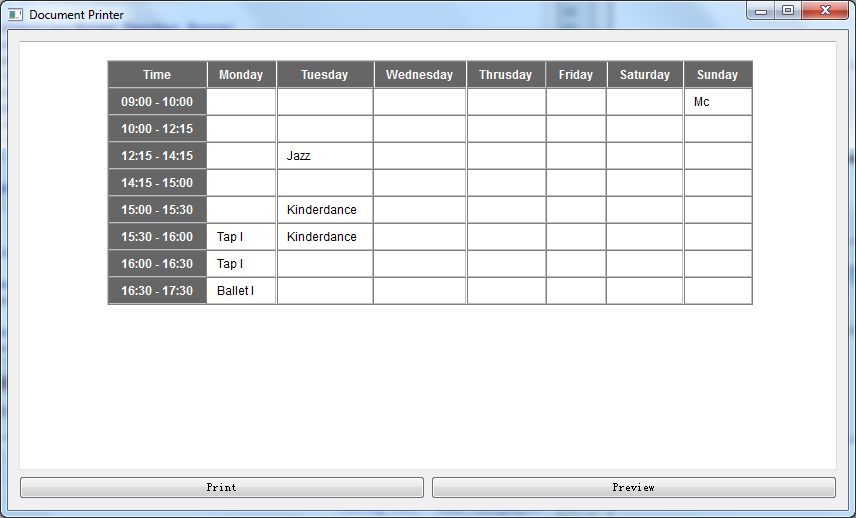
\includegraphics[scale=0.5]{pics/schedule_dialog.png}\\
User can see schedule of each teacher/student which is dynamically generated by the algorithm. User can preview those information in a pdf or print it out in the printer.\\

\subsubsection{Change Password/Username}
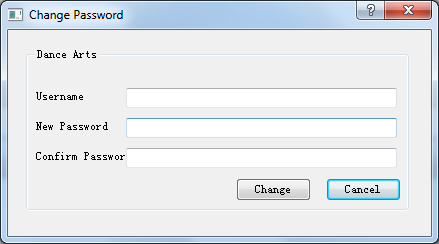
\includegraphics[scale=0.5]{pics/change_pass.png}\\
This dialog allows current users to change their password/Username.\\



\section{Database}

\subsection{Technologies  Used}
The database the team used was MySQL

\subsection{Component  Overview}
The database tables are listed below.


\subsection{Phase Overview}
This is an extension of the Phase Overview, but specific to this component. 
It is meant to be basically a brief list with space for marking the phase status.

\subsubsection{Initial creation}
There are Student, teacher, admins and class tables and each are connected by different relationship in order to perform certain functionality we want. It consists many-to-many relationship has intermediate table and many-to-one relationship. We also have N account table for user authentication and it has permission level included in order to distinguish different user groups for example admin and teacher have different permission levels.\\

\subsubsection{Later creation}
The database will need to be updated as further iterations of the DanceSoft project are created.


\subsection{ Architecture  Diagram}

 
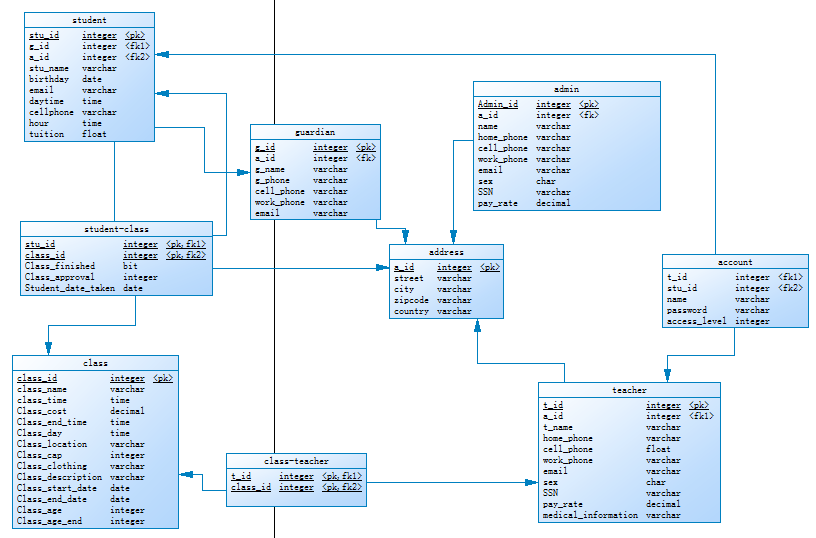
\includegraphics[scale=0.8]{pics/database.png}\\

\subsection{Data Flow Description}
Each table has different purposes for example teacher's table is for storing information of teachers and student's table's is for storing information of student. Different tables are evoked by different functionality for instance the function of search for students' information will use student and guardians and address tables at same time, and for assign teacher to classes it will use teacher and class and class-teacher table at same time


\subsection{Design Details}
We first draw row diagram on board and try to figure out which table is necessary to implement and did some fine pruning. later stage, we create this scheme in power designer and create ERP diagram. From that diagram, we create our initial scheme and generate it in MySQL database. We also add couple of new tables on the fly due to the project needs such as the payment tables. For example, we add payment and payrate table for pay roll purpose, and System table for distinguish different semester in order to produce correct result of each function. The discount and credit are also added based on various needs.

\subsubsection{Account table}
Store account's information of admins, teacher and students.\\
\textbf{t\_id:} foreign key which links teacher and account table together\\
\textbf{admin\_id:} foreign key which links admin and account table together\\
\textbf{name:} username\\
\textbf{password:} password\\
\textbf{access\_level:} different user's group has different access level

\subsubsection{Address table}
Store address of admins, teacher and students\\
\textbf{id:} This is a primary key and store address id.\\
\textbf{street:} Store information of street.\\
\textbf{city:} Store information of city.\\
\textbf{zipcode:} Store information of zipcode.\\
\textbf{country:} Store information of country.\\


\subsubsection{Admin table}
Store information of admins\\
\textbf{admin\_id:} Store admin's id\\
\textbf{admin\_name:} Store admin's name\\
\textbf{admin\_home\_phone:} Store admin's hone phone number\\
\textbf{admin\_cell\_phone:} Store admin's cell phone number\\
\textbf{admin\_work\_phone:} Store admin's work phone number\\
\textbf{admin\_email:} Store admin's email address\\
\textbf{admin\_sex:} Store admin's sex\\
\textbf{admin\_ssn:} Store admin's social security number\\
\textbf{admin\_pay\_rate:} Store pay rate of admin

\subsubsection{Class table}
Store classes' information\\
\textbf{class\_id:} This is a primary key store class' id\\
\textbf{class\_name:} Store the name of class \\
\textbf{class\_time:} Store the starting time of class\\
\textbf{class\_end\_time:} Store the ending time of class\\
\textbf{class\_cost:} Store the price of the class\\
\textbf{class\_day:} Store which day has class\\
\textbf{class\_location:} Store the location of class\\
\textbf{class\_cap:} Store the capacity of class\\
\textbf{class\_clothing:} Store the clothing requirement of class\\
\textbf{class\_description:} Store the class' description\\
\textbf{class\_start\_date:} Store the start date of class\\
\textbf{class\_end\_date:} Store the end date of class\\
\textbf{class\_age:} Store the starting range of class age allowed\\
\textbf{class\_age\_end:} Store the ending range of class age allowed

\subsubsection{Credits table}
Store student's credit\\
\textbf{credit\_id:} This is a primary key store credit' id\\
\textbf{student\_id:} Store the id of student \\
\textbf{credit\_amount:} Store the amount of credit student have\\

\subsubsection{Discount table}
Store discount policy\\
\textbf{student\_id:} This is a primary key store student' id\\
\textbf{is\_annual:} Store is annual payment \\
\textbf{is\_early:} Store is early bird\\
\textbf{semester:} Store which semester being paid\\

\subsubsection{Guardian table}
Store guardians' information\\
\textbf{g\_id:} This is a primary key store guardian id\\
\textbf{a\_id:} This is a foreign key links guardian and address tables together\\
\textbf{g\_name:} Store the name of guardian\\
\textbf{g\_phone:} Store guardian's phone number \\
\textbf{g\_work\_phone:}Store guardian's work phone number\\
\textbf{g\_email:} Store guardian's email

\subsubsection{One\_Off\_Fees table}
Store entry's of fees\\
\textbf{fee\_description:} This is a primary key store description of fees\\
\textbf{fee\_cost:} Store the cost corresponding to fees\\

\subsubsection{Payment table}
Store individual payment for each student \\
\textbf{payment\_id:} This is a primary key store id of payments\\
\textbf{student\_id:} This is a foreign key store id of students\\
\textbf{amount\_paid:} Store amount of paid of each payment\\
\textbf{semester\_paid:} Store semester paid for each payment\\
\textbf{date\_paid:} Store date paid for each payment\\
\textbf{method:} Store different payment method\\

\subsubsection{Payrate table}
Store different pay rate of each category\\
\textbf{payrate\_id:} This is a primary key store id of payrates\\
\textbf{payname:} Store different payment's name\\
\textbf{payrate:} Store different payrate\\


\subsubsection{Student table}
Store students' information\\
\textbf{stu\_id:} This is a primary key store student's id\\
\textbf{g\_id:} This is a foreign key links guardian and student tables together\\
\textbf{a\_id:} This is a foreign key links student and address tables together\\
\textbf{stu\_name:} Store student name\\
\textbf{birthday:} Store student birthday\\
\textbf{email:} Store student email\\
\textbf{daytime:} Store available time of student\\
\textbf{cellphone:} Store student cell phone number\\
\textbf{hour:}Store hours of classes student is taken\\
\textbf{tuition:} Store student unpaid tuition\\


\subsubsection{Teacher table}
Store teachers' information\\
\textbf{t\_id:}This is a primary key store teacher's id\\
\textbf{a\_id:}This is a foreign key links address and teacher tables together\\
\textbf{t\_name:} Store teacher's name\\
\textbf{home\_phone:} Store teacher's hone phone number\\
\textbf{cell\_phone:} Store teacher's cell phone number\\
\textbf{work\_phone:} Store teacher's work phone number\\
\textbf{email:} Store teacher's email address\\
\textbf{sex:} store teacher's sex\\
\textbf{ssn:} Store teacher's social security number\\
\textbf{pay\_rate:} Store teacher's pay rate\\
\textbf{medical\_information:} store teacher's medical information


\subsubsection{Student\_Class table}
Link student and class tables together\\
\textbf{stu\_id:} This is a foreign key and primary key links student and student-class tables together\\
\textbf{class\_id:} This is a foreign key and primary key links class and student-class tables together\\
\textbf{class\_finished:} Store whether student finished this class\\
\textbf{class\_approval:} Store whether student get approved for this class\\
\textbf{stu\_data\_taken:} Store when student took the class

\subsubsection{Teacher\_Class table}
Link teacher and class tables together\\
\textbf{t\_id:} This is a primary and foreign key links teacher and teacher-class together\\
\textbf{class\_id:} This is a primary and foreign key links class and teacher-class tables together 

\subsubsection{System table}
Store semester's information.\\
\textbf{system\_id:} This is a primary store id of each semester\\
\textbf{term:} Store terms\\
\textbf{current\_information:} store current semester

\subsubsection{Teacher\_Payrate table}
Link teacher and payrate together\\
\textbf{teacher\_id:} This is a foreign key and primary key links teacher and teacher-payrate tables together\\
\textbf{payrate\_id:} This is a foreign key and primary key links payrate and teacher-payrate tables together\\
\textbf{hours:} Store hours for teacher actually worked.

\subsubsection{Tuition\_Rates table}
Link teacher and payrate together\\
\textbf{tuition\_description:} This is a primary key stores description of tuition\\
\textbf{tuition\_rate:} Store tuition rate of each description\\
\textbf{tuition\_time:} Store tuition time of each description
